\section{Keywords}
{\it Computer vision, Object recognition, Brand logo detection, Graphical processing unit, Effectiveness of brand logo, Brand logo in advertisement clips, Brand logo in movies, GPU based computation, Cluster of GPUs.}
  
\section{Background}

Advertisement is defined as a medium of publicizing or promoting an event, product or service in public in the form of notice or announcement \cite{adver7:online}. It can be in the form of short video clips, brand logo images, text based banners and various other forms. Due to the advent of digital media technology, most of the advertisement and process of brand awareness creation has been revolutionized in large extent.\\ \\
Brand logo based advertisement is one of the many forms of advertisements using digital media. It is defined as the graphical representation of a company, people or an organization \cite{What3:online}. Embedded marketing is the form of advertisement which lacks ads in explicit form \cite{baig2013contemporary}. But it contains relevant information in the form of embedded entities such as brand logos in the main content such as movies, short clips, news or sport event \cite{baig2013contemporary}. Placement of brand logos in short video clips, movies and sport events is the most prevalent form of embedded marketing and it has been vastly benefited with the advent of digital media technology 	\cite{baig2013contemporary}.\\ \\
One more important aspect of embedded brand logo marketing is to determine the effectiveness of its placement in the main content. The brand logo placement in a movie plays an major role in determining its effectiveness \cite{JCOM}. The position of the brand logo, its timing, visibility time, its reference with the story line and of course the popularity of the event or movie influences the viewers to remember the brand logo in their implicit memory \cite{JCOM}. Determining the value of effectiveness of a brand logo in a video sequence of a live event is a challenging task. The detected brand logos and its effectiveness determines the advertising value of a video sequence of a live event. This information is used by the companies to rethink their brand logo design and placement in a live event situation or in a movie.\\ \\
Any application developed has to be executed on the hardware that provides favorable architecture for computation. The task of detecting brand logos in input video stream can be accelerated using parallel SIMT (Single instruction multiple thread) cores of graphical processing units. GPUs offer a large amount of computation power for the applications that have feature of data parallelism. Since most of the image and video processing algorithms perform same operation to large amount of data, a lot of speed up can be achieved in terms of execution time. For example, filtering operation is about performing a similar function on a large amount of pixels in an image. Hence choosing a right architecture to perform task of brand logo detection is of utmost importance.        

\section{Problem}
The process of detecting objects and patterns in live video sequence is a challenging task. The occurrence of brand logos in different size, shape, rotation angle, skewness and due to presence of occlusion \footnote{In all rendering algorithms there is a chance of creating holes that cannot be reconstructed in the computed images, or overlapping pixels that cannot be interpreted. This phenomenon is defined as occlusion \cite{Depth6:online}.} effects makes the detection of brand logos in a input video stream a daunting task. But there is a dire need of automating the process of brand logo detection and measurement of effectiveness of the same in video sequences. The reason is due to the fact that manual detection and characterization of brand logo in live video sequence is an arduous and error prone task. One more reason is that by automating the task of brand logo detection in live video stream or in humongous amount of stored movie data a lot of human effort can be avoided.  


\section{Problem Statement}
There is a need for an application that determines the effectiveness of brand logo in a video sequence. This information is used by the companies to understand the effectiveness of the brand logo as viewed by the target audience.To be precise the problem that will be addressed in this project is \\ \\ 
{\it "To detect and measure effectiveness of brand logo of a company in a video sequence, as viewed by the viewers using GPU cluster."} 

\section{Purpose}
The purpose of the project is to develop an application that enables companies to measure the effectiveness of their brand logo in a video sequence in real time. The effectiveness of a particular detection can be measured based on position of the detected logo, brightness and clarity of the logo in general. This information can be used by the companies to understand the effectiveness of their logo as perceived by their viewers. This feedback will help the companies to rethink their strategy of designing the logo, and to make it more appealing to the viewers in future.

\section{Goals of the project}

The aim of the project is to develop an application that automatically detects logos of famous brand names in an input video stream. The detected information can be further used by the advertisement engine to select and present the advertisement corresponding to the detected brand logo in the video stream. The algorithm that detects the brand logo will be executed on cluster of graphical processing unit (GPU) to enable real time detection of brand logos.

Further, the goals of the project have been categorized into compulsory and optional goals.  

\subsection{Compulsory goals} 
\begin{itemize}
	\item To research about related work and compare various algorithms used for brand logo detection. Choosing an optimal algorithm for the implementation of brand logo detector.
	
	\item To develop a GPU based brand logo detector in an input video stream.
	
	\item To enable multiple brand logo detection in a single frame of input video.
	
	\item To accelerate developed real time brand logo detector using multiple GPUs.
	
	\item To develop a metric, as perceived by the user to define effectiveness of a brand logo in a video sequence.   
\end{itemize} 

\subsection{Optional goals}
\begin{itemize}
	\item To develop an application framework, which accepts video sequence encoded in any format and detects brand logo in the video sequence.     
	
	\item To analyze the effectiveness of brand logo in movies, the metric of effective has to be extended to involve several factors like popularity of the movie, positioning of the brand logo and popularity of the actors and the scene involving brand logo. 
	
\end{itemize}     
 
\section{Method}
  
  In the domain of scientific research, there exists many methods that could be used to conduct research to arrive at a conclusion about a topic and also to answer a research question. Foremost step of the process is to determine the type of research method that will be used in the thesis project. Deciding upon a research method involves careful analysis of question to be answered, availability of data, nature of the data and the process of obtaining datum required for deriving the results and conclusion. The process of defining a problem statement involves, in depth understanding of the current research in the area of interest. Literature study in the area of interest will be performed to get valuable insights about unsolved problems, it also provides necessary knowledge for understanding the recent developments in the field. 
  \\ \\
  During the literature study phase of the master thesis, qualitative methodology as mentioned in \cite{haakansson2013portal} will be used to understand the current problems in the field of research. Research approach would be of inductive in nature to understand the influence of various variables in the context of answering the research question. Inductive approach is suitable in the context of current research question, since in this approach data is collected with exploratory research strategy to determine the relationship between the variables and the phenomenon \cite{haakansson2013portal}. The research question of finding an optimal algorithm for brand logo detection in video stream requires understanding of various variables namely efficiency of the algorithm, accuracy rate of detection, implementation feasibility and many more factors. Hence the task of determining optimal algorithm can be carried out by exploratory research to determine the relationship between the variables \cite{haakansson2013portal} by means of surveying the previous work in the field. The objective of the surveying previous work is to find the optimal algorithm for detection task and the reasons for choosing the same in the given context.         
  \\ \\
  Further, the focus of the project is to improve the current state of the art algorithm method to solve the practical problem of detecting brand logos in video stream. In order to accomplish the task, method of applied research under quantitative research methodology \cite{haakansson2013portal} will be used. The methodology of applied research deals with solving practical problems as the one in question. It is a type of research methodology that benefits from previously researched methods in the field of interest to construct further to solve a practical problem. Since the problem statement in focus has been a long standing issue in the area of computer vision, the research work can be benefited from the results obtained from work of earlier researchers in this field \cite{haakansson2013portal}. 
  \\\\
  The research approach adopted for this task is of deductive in nature, in this method various experiments are conducted in order to collect data during the detection task in a video stream. Collected data is analyzed to obtain valuable metrics such as mean average accuracy of detection, time taken for detection,false detection rate, effectiveness measure of the logos in the set of validation video streams. Deductive approach fits perfectly for the research question , since it involves various variables and also there is a need for understanding causal relationship among them.    
  Data presentation is the process of representing the collected data during the process of research using graphs, text and tables. Also it will be ensured that the collected data and results are repeatable and reliably documented in the report.  
 
\section{Milestone chart (time schedule)}
 \begin{figure}[htp] \centering{
 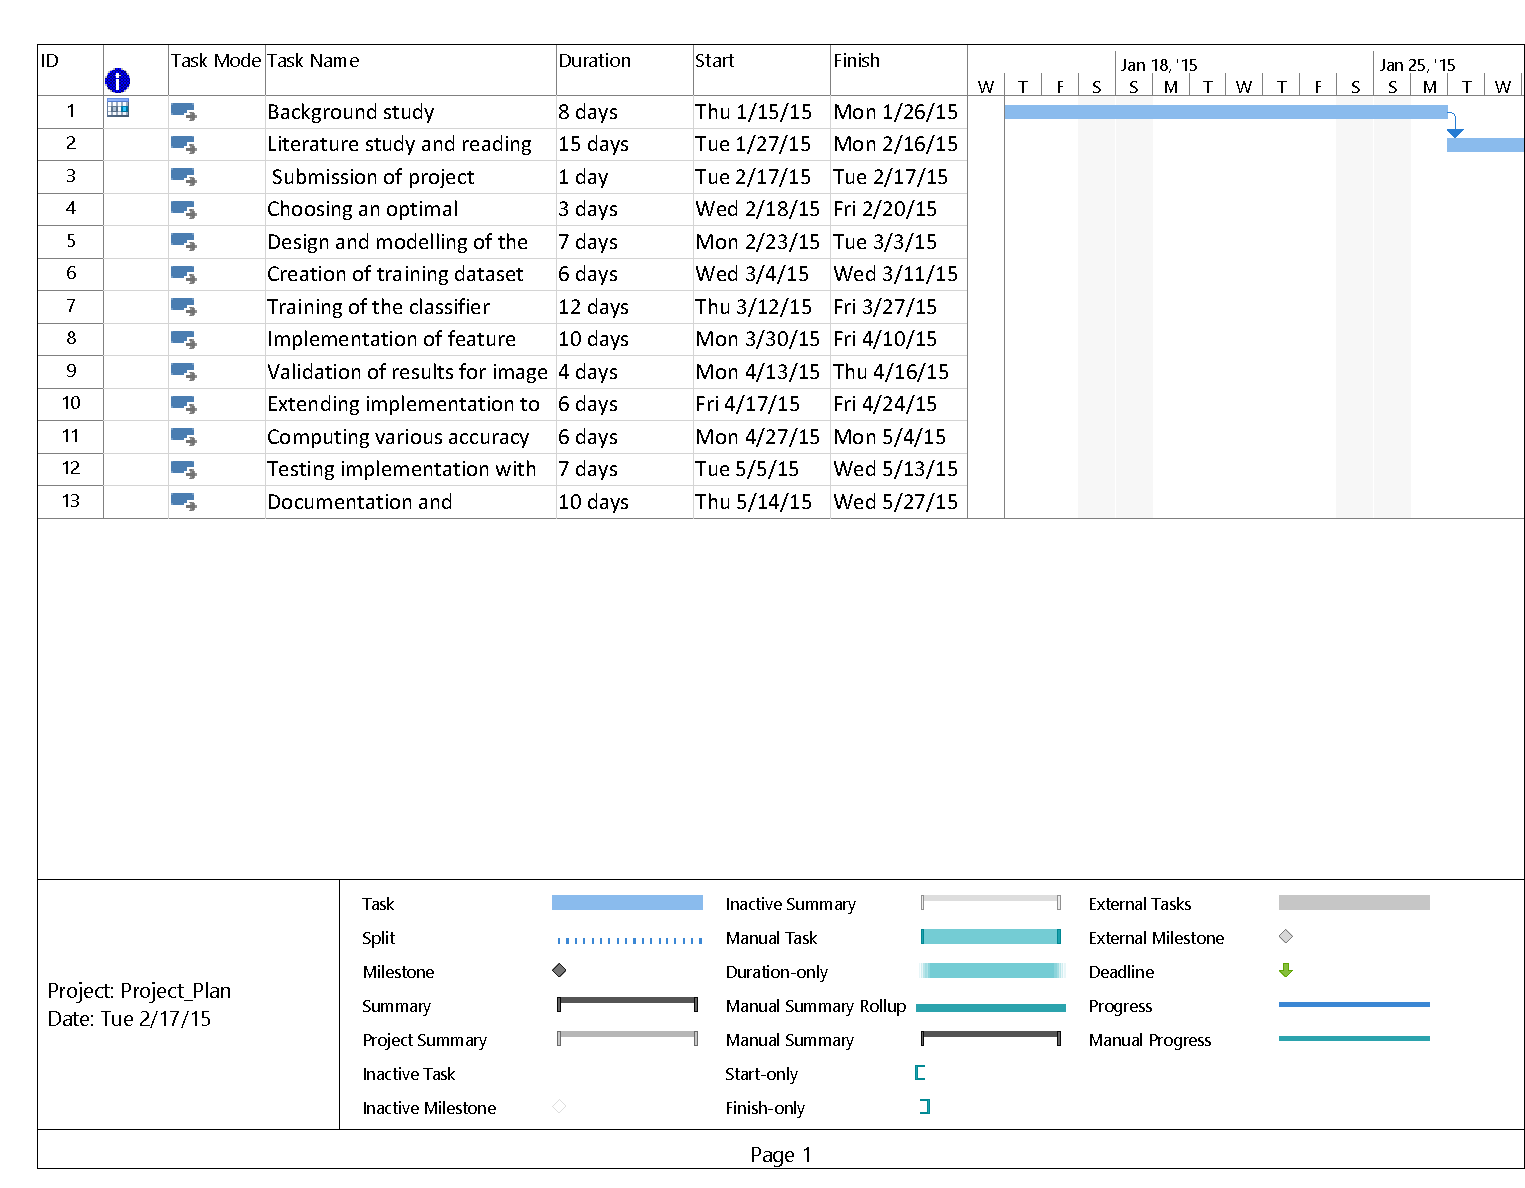
\includegraphics[scale=0.72]{./TeX_files/Project_Plan}}
 \caption{Project plan timeline}
 \end{figure}

 \newpage
 \section{Risk, Consequences and Ethics}
 \begin{figure}[htp] \centering{
 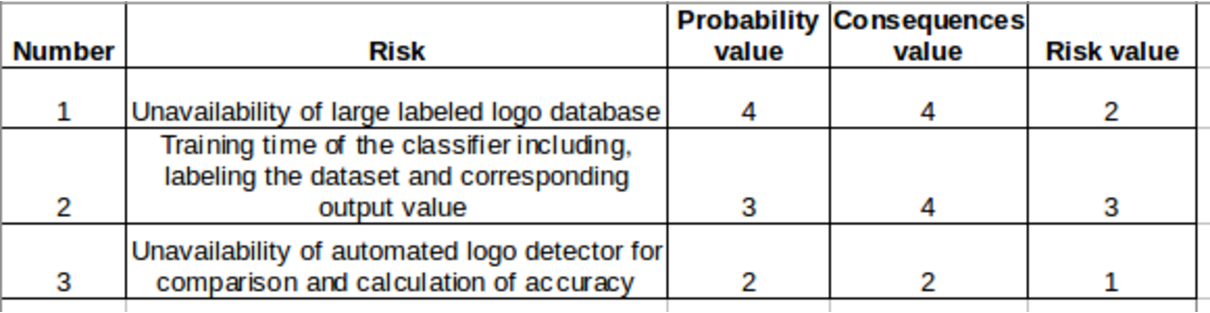
\includegraphics[scale=0.5]{./TeX_files/risk_1.pdf}}
 \caption{Risk analysis}\label{fig:risk}
 \end{figure}

%\section{Risks, Consequences and Ethics}
 For all experiments conducted the collected data will be ensured to be repeatable and reliable. The actual details of architecture and parameters will be presented as part of the report to allow repeatability of the experiments on the validation dataset. \\
 The risks involved in the project are as tabulated in figure \ref{fig:risk}. All the values in the table are in the range 1-4, with 4 being the highest scale. Due unavailability of large labeled logo dataset in the internet, this risk is considered with the highest value of probability of risk and consequence for the project. Likewise, the task of brand logo detection requires training of the classifier to perform classification of the detected logos in the video stream and it takes approximately a week time due to the large set of  training samples on graphical processing unit (GPU). It also requires manual labeling of the training samples and the corresponding output label. \\
 One more task that needs attention and time, is creation of reference database containing information about the logos in validation set of videos. Later this data is used to compare with the obtained results to compute mean average accuracy and other related parameters.\\
 The necessary action required to reduce the risk involved in the project is also tabulated in figure \ref{fig:action}
 
 \begin{figure}[htp] \centering{
  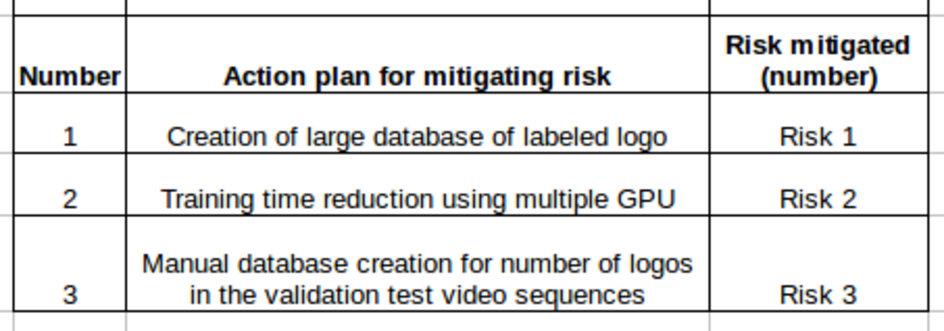
\includegraphics[scale=0.76]{./TeX_files/action_1.pdf}}
  \caption{Proposed mitigation actions}\label{fig:action}
 \end{figure}
 
 In order to reduce the risks involved in project, there are few mitigation action plans proposed. First and most important, is to create a labeled database of various logos with corresponding output values. 
 
\pagebreak
\section{Summary}
Nowadays, most of the advertising carried out by industry to promote their products and to convince the viewers is based on video. All the registered companies have their personalized brand name logo to capture the attention of the customers. Brand name logos also entices viewers to remember company's brand name, and this further helps the companies to sell their products in large quantities. Due to the invasion of powerful hand held devices the trend in video based advertising is highly benefited. Short video clips in the form of advertisements are presented to the customers for purpose of marketing and brand name awareness.    
